\section { Design }

\subsection{Multithreading}
In order to maximise ease-of use, the software should have a graphical user environment (GUI) so that the current audio being played can be easily visualised (in-line with objective 2). The program will use a multithreaded model, with a separate "audio thread" and "GUI thread", allowing the two to run concurrently without blocking each other's processing.

\begin{figure}[h]
	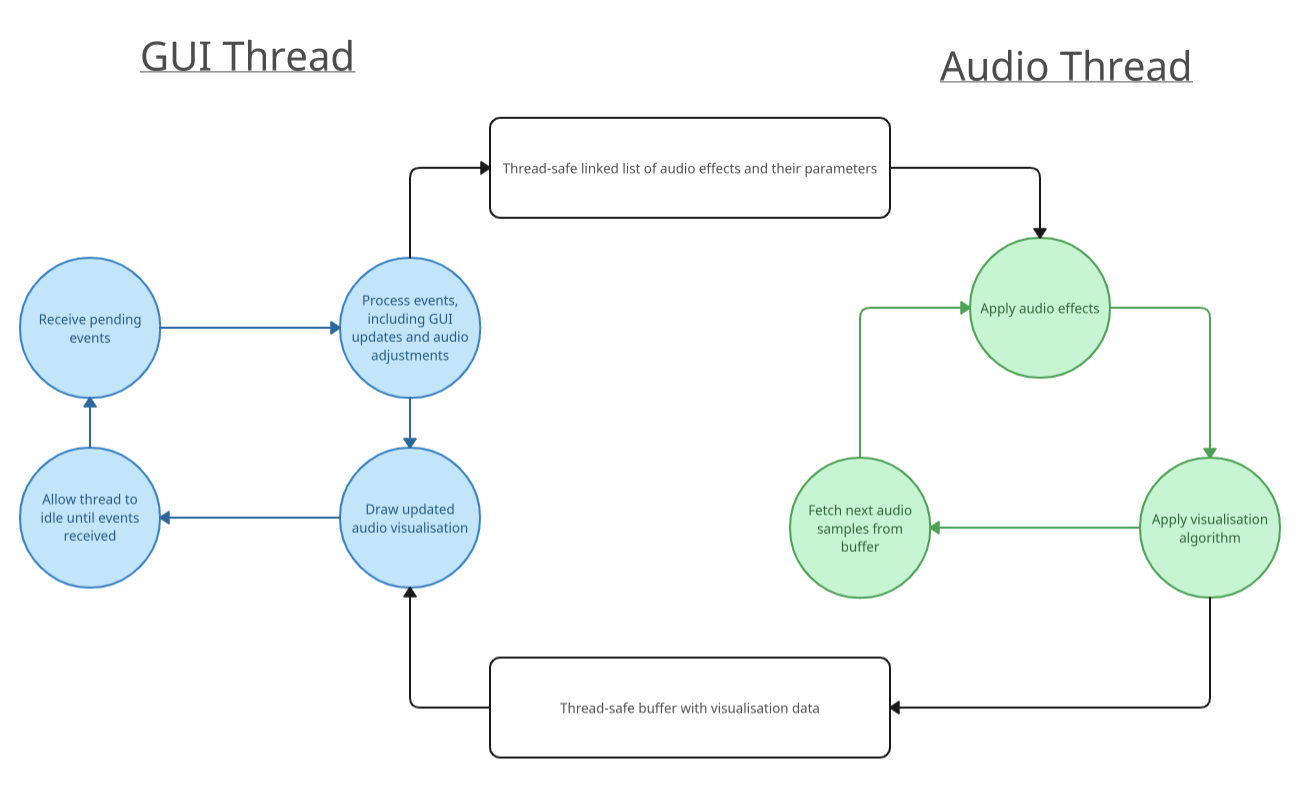
\includegraphics[width=17cm]{threading}
	\caption{Inter-thread diagram - see below for justification for thread-safe data structures}
\end{figure}

\paragraph{}
Typically, GUI programs are written using an event-based paradigm that minimises CPU idle-time. The consequence of this is that, for most of the time, the GUI thread is suspended, awoken only when events from the user (such as mouse clicks or resizing the window) "wake it up". This is desirable in order to minimise system resources used, as more CPU-time will be available for the audio processing requirements, helping to reach the real-time requirements of objective 6. However, this presents a unique challenge. With a single-threaded model:
\begin{itemize}
	\item If the event-based model is followed, the GUI thread is only active when there are pending GUI events to be processed, meaning audio processing can only occur sporadically (resulting in "non-constant" audio)
	\item If instead the GUI thread is constantly active processing audio it will never reach a point where it can process pending events, meaning the program will hang and refuse to process inputs.
\end{itemize}

Hence it is desirable to split the program into two distinct threads. The audio thread can play the audio and perform all necessary processing tasks, whilst the GUI thread can relay input parameters and commands to the audio thread (such as "switch song", "apply effect", etc.).

\paragraph{}
To avoid race conditions\footnote{
	 Race conditions occur when one thread tries to read data whilst the other writes to it. If, for example, the GUI thread removed an audio effect from the audio effect list (see above) and freed it from memory whilst the audio thread was applying that same effect, the audio thread would suddenly be reading from invalid memory, likely resulting in a crash or undefined behaviour.
}, the data that is read by both threads should be thread-safe - only one thread should be able to access the data at a time. This can be achieved by using mutexes\footnote{
	A mutex is an object that prevents multiple threads from accessing data at the same time. It can be thought of as a lock, which can only be unlocked for one thread at a time. They are preferable to spinlocks as they do not require the CPU to waste cycles waiting for the data to be "unlocked", as instead the thread can suspend itself until the mutex becomes available.
}.

\subsubsection{Audio Effects Data Structure}
\paragraph{Picking a data structure} The user will likely want to adjust the order of audio effects at will, and as the same time, it must be very fast to insert and  remove audio effects so as to minimise the time spent not processing audio (even a very short pause may result in "crackles" on weaker hardware). To solve this problem, the audio effects can be stored in a linked list, as unlike std::vectors (dynamic C++ arrays) they prove fast insertion, deletion and swapping irrespective of the number of elements stored.

\paragraph{Making it thread-safe}
To satisfy the requirements of multithreading (see above), I will write my own custom "atomic linked list", backed by a mutex\footnote{
	See above footnote on mutexes
}, which will function just like a normal linked list but maintain thread-safety in all its operations.


\pagebreak
\subsection{Audio Effects Architecture}
The full list of audio effects detailed in the analysis section is as follows:
\begin{itemize}
	\item Equaliser (frequency modification) - selectively modifying frequencies such as by performing a bass boost
	\item Echo - making audio sound like it's recorded in a large room
	\item Volume adjustment - modifying the amplitude of the audio
	\item Noise - adding subtle imperfections to the audio
\end{itemize}

\subsubsection{Unique Audio Effect Traits}
Each audio effect will need its own properties, and potentially its own mutable state (for example, the echo effect needs to "remember" the previous audio samples so it can repeat them later). Below is a summary of the requirements, properties and state of each audio effect.

{
\renewcommand{\arraystretch}{1.5}
\begin{table}[h!]
	\begin{center}
		\begin{tabularx}{1.0 \textwidth} {
				| >{\raggedright\arraybackslash}X 
				| >{\raggedright\arraybackslash}X
				| >{\raggedright\arraybackslash}X 
				| >{\raggedright\arraybackslash}X  |
			}
			\hline
			Effects & Requirements & Properties & State \\
			
			\hline
			Equaliser & Allow the user to alter the volume of a selected frequency range. Multiple equaliser effects can be applied successively to cover multiple ranges.  & Lower frequency \newline  Upper frequency \newline Multiplier  & None \\
			
			\hline
			Echo & Produce an echo effect where audio sounds like it's getting reflected in a large room & Fall-off (how quickly echoes fade) \newline Delay samples (how many samples must pass before a sample is echoed) & Previous audio samples buffer \\
			
			\hline
			Volume & Adjust the volume / amplitude of incoming audio & Volume multiplier & None \\
			
			\hline
			Noise & Add subtle imperfections to the audio & Intensity (the volume of the noise) & None\\
			
			\hline
		\end{tabularx}
	\end{center}
\end{table}
}

\subsubsection{Common Audio Effect Traits}
Immediately it is obvious that all audio effects will share many common features. Each effect shall:
\begin{itemize}
	\item Take a number of audio samples as input
	\item Have a number of configurable options which need to be exposed to the GUI front-end
	\item Perform processing on all audio samples at once
	\item Output its final processed audio
\end{itemize}

\paragraph{}
Given these requirements it is wise to use an object-orientated inheritance approach where effect subclass inherits from a common parent, which provides common functionality (such as the storage and exposing of configuration options), as well as providing a common interface that other parts of the code can use. In order to abstract away the details of interacting with an audio effect, two new classes will also be needed.

\subparagraph{Packet} A packet represents a chunk of audio awaiting processing by the effect. However, some effects require knowledge of both the previous audio samples and future audio samples (like echo). Thus, each packet will consist of 3 audio buffers - one for the previous, current and next buffer of audio samples. A packet will also contain the frequency of the incoming audio as this is required for the FFT maths.

\subparagraph{Property} Each audio effect has a number of configurable properties. To aid in validation, each property will have a current,  minimum and maximum value, as well as a flag to differentiate between integer values and decimal values.

\paragraph{}
Both these classes will be independent of the main audio effect parent class. The audio effect parent class will merely use these classes to represent the data provided and stored by it. This is an example of {\it composition}.

\subsubsection{Properties Data Structure}
Each audio effect will have a list of properties. When drawing a properties GUI, the front-end code will want an easy and convenient way of both getting a list of all available properties, along with their respective names. In a similar fashion, when setting the values of certain properties, it will be most convenient if properties can be accessed using their names.

\paragraph{}
I will use a hash-map as my data structure for this purpose. Hash-maps can be indexed by using the name of the property (e.g. "minimum frequency" as the key), simplifying the front-end code and avoiding the need for a separate "property name" variable. In addition, they provide very fast look-up with an O(1) time. Whilst hash-maps are expensive when it comes to adding and removing elements, each audio effect will only have a fixed number of properties so this will not be an issue.

\subsubsection{UML Class Diagram}
After considering all the requirements of the multiple classes required, I have constructed a class diagram. However, a slight modification has been made to the typical UML structure: properties of audio effects are prefixed with an * (asterisk) in order to indicate that their are not attributes {\it per se}, but rather are elements in their parent's properties hashmap.

\begin{figure}[h]
	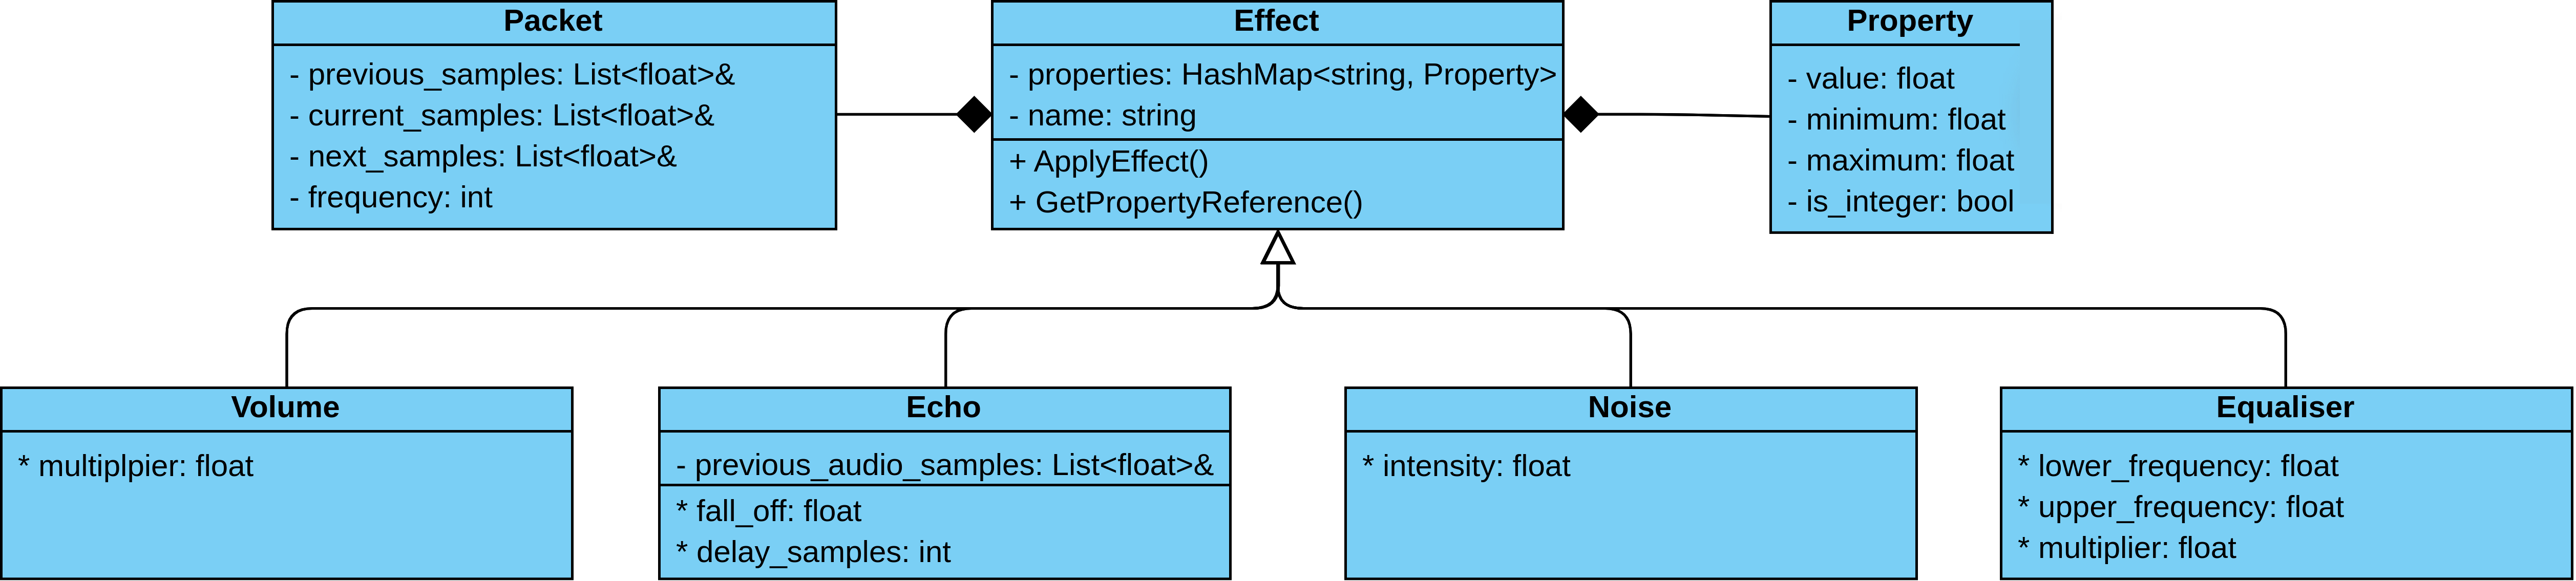
\includegraphics[width=\textwidth]{effects class diagram}
	\caption{UML class diagram containing attributes, operations and custom "properties"}
\end{figure}

\pagebreak

\subsection{High-Level Audio Effects Flowcharts}
\begin{figure}[H]
	\subsubsection{Equaliser}
	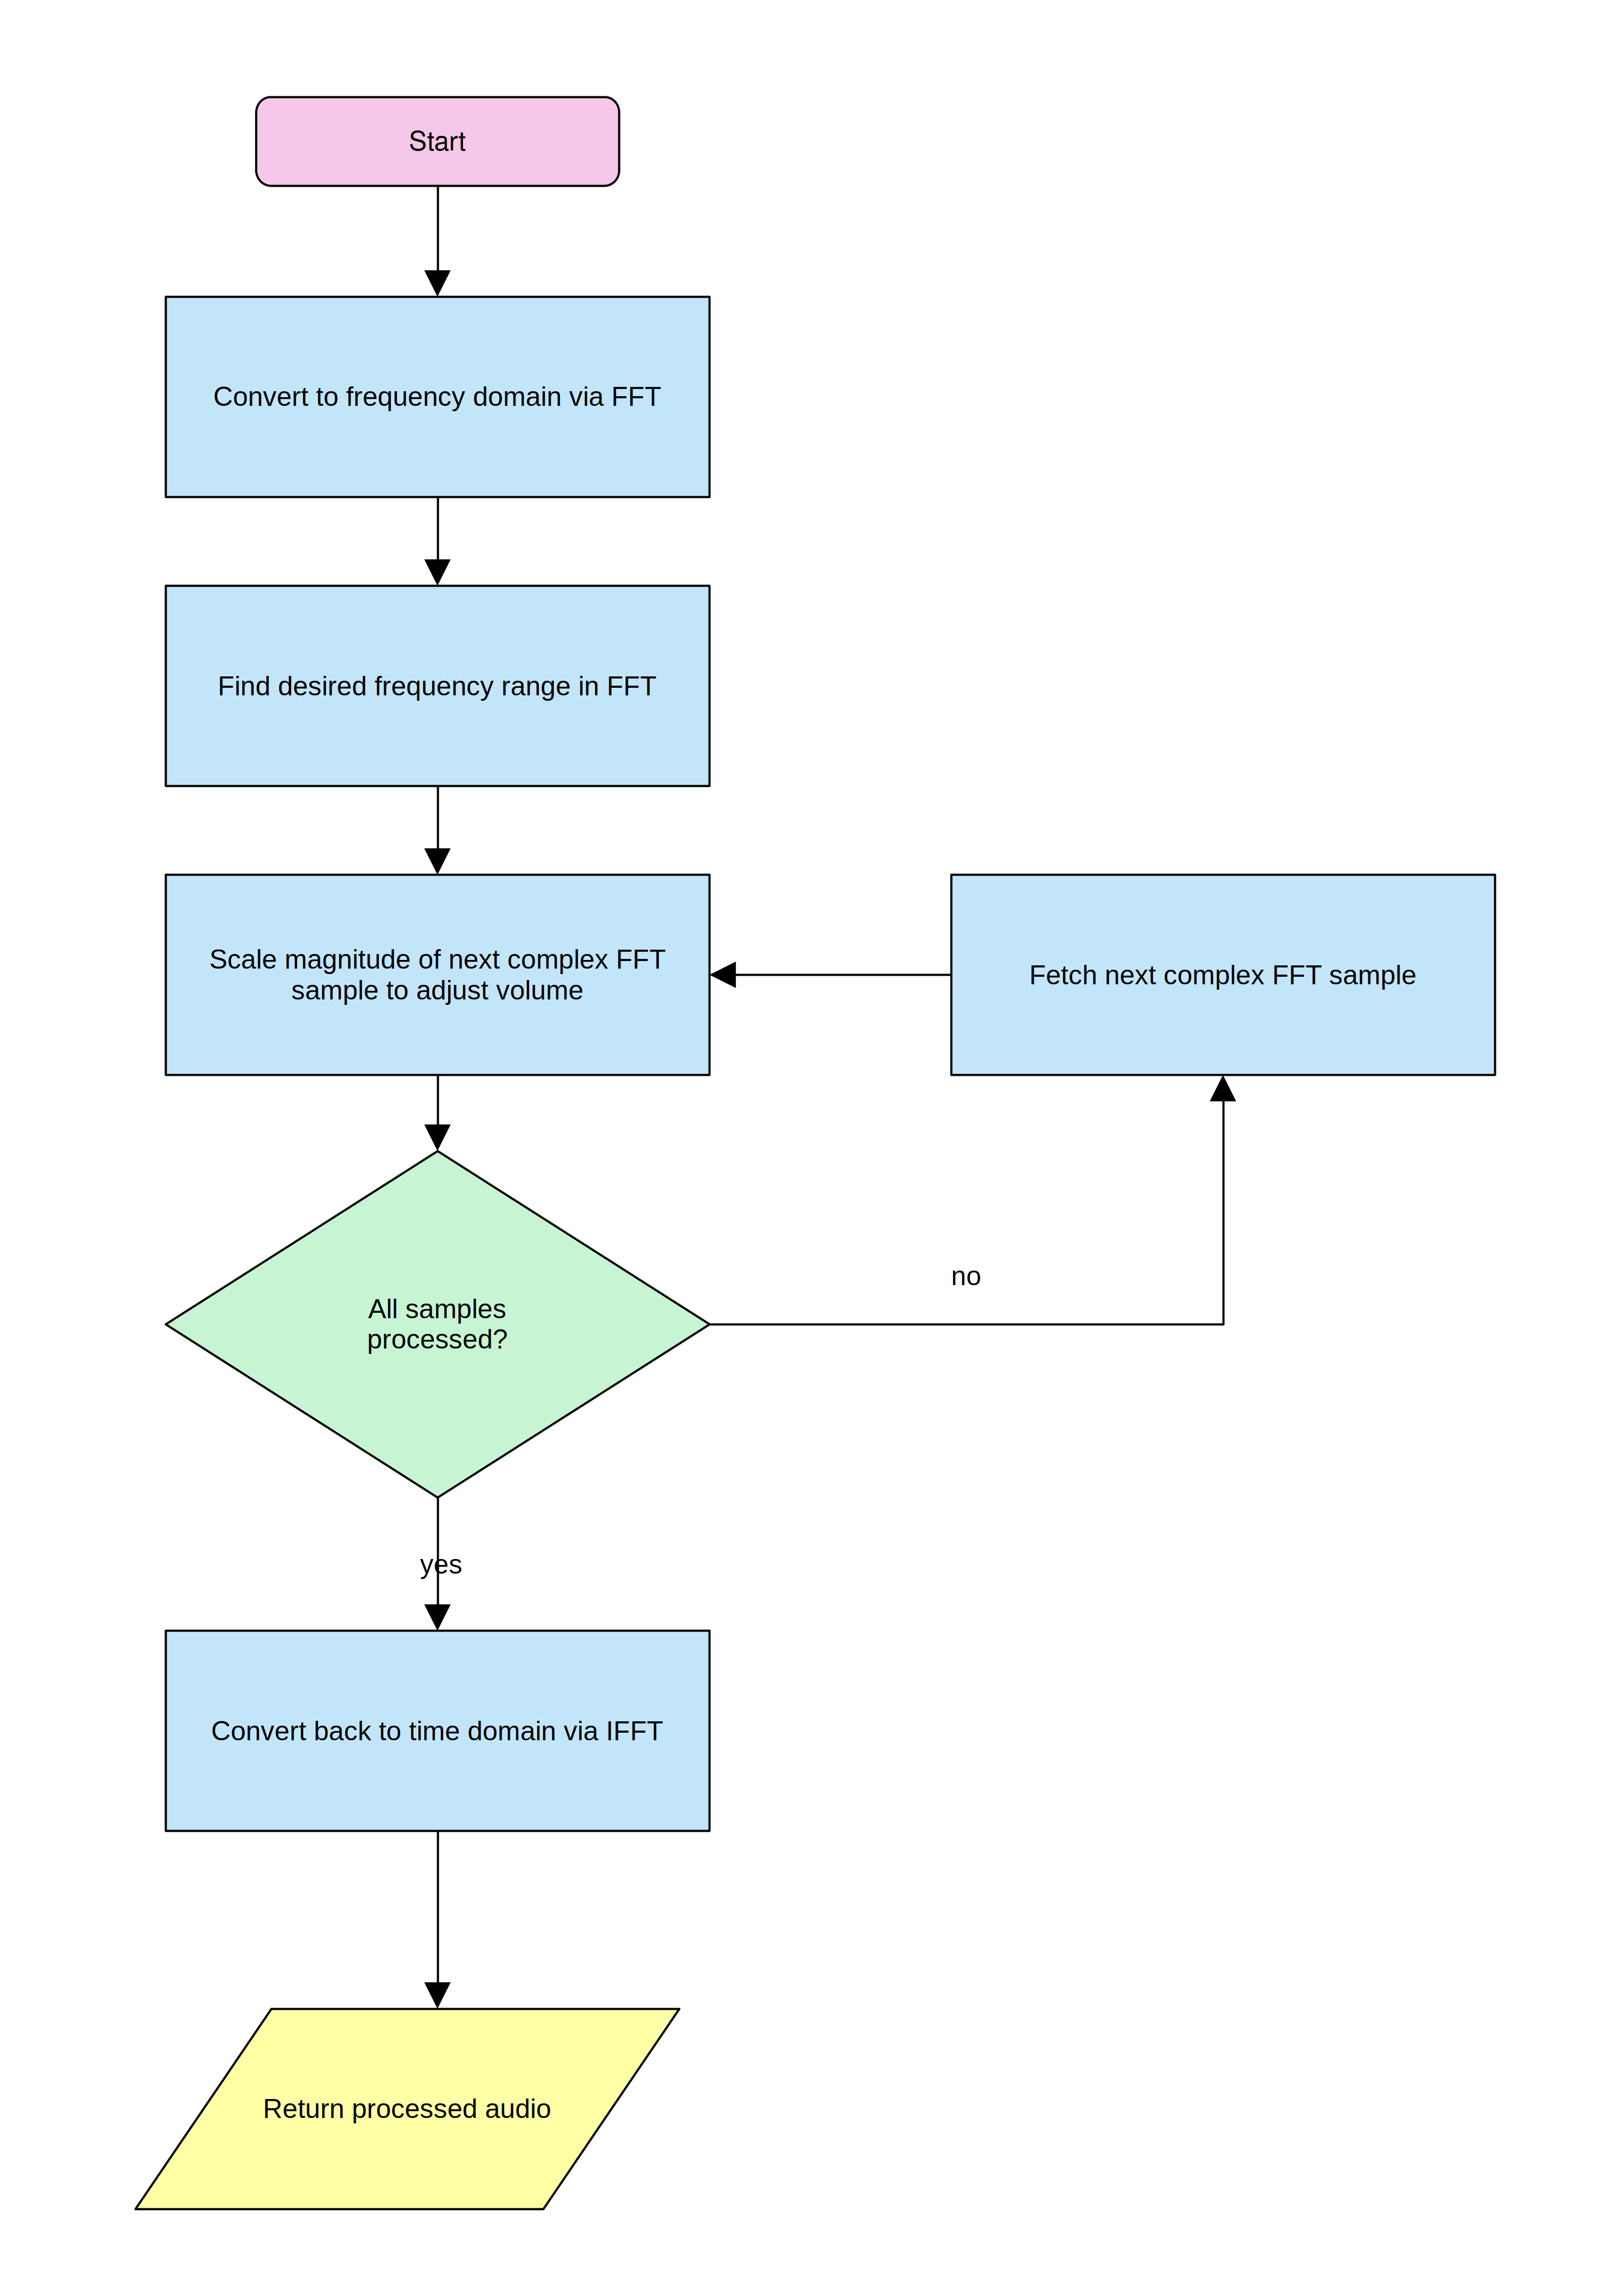
\includegraphics[width=14cm]{equaliser flowchart}
	\caption{Flowchart for equaliser (frequency modification) audio effect}
\end{figure}

\begin{figure}[H]
	\subsubsection{Echo}
	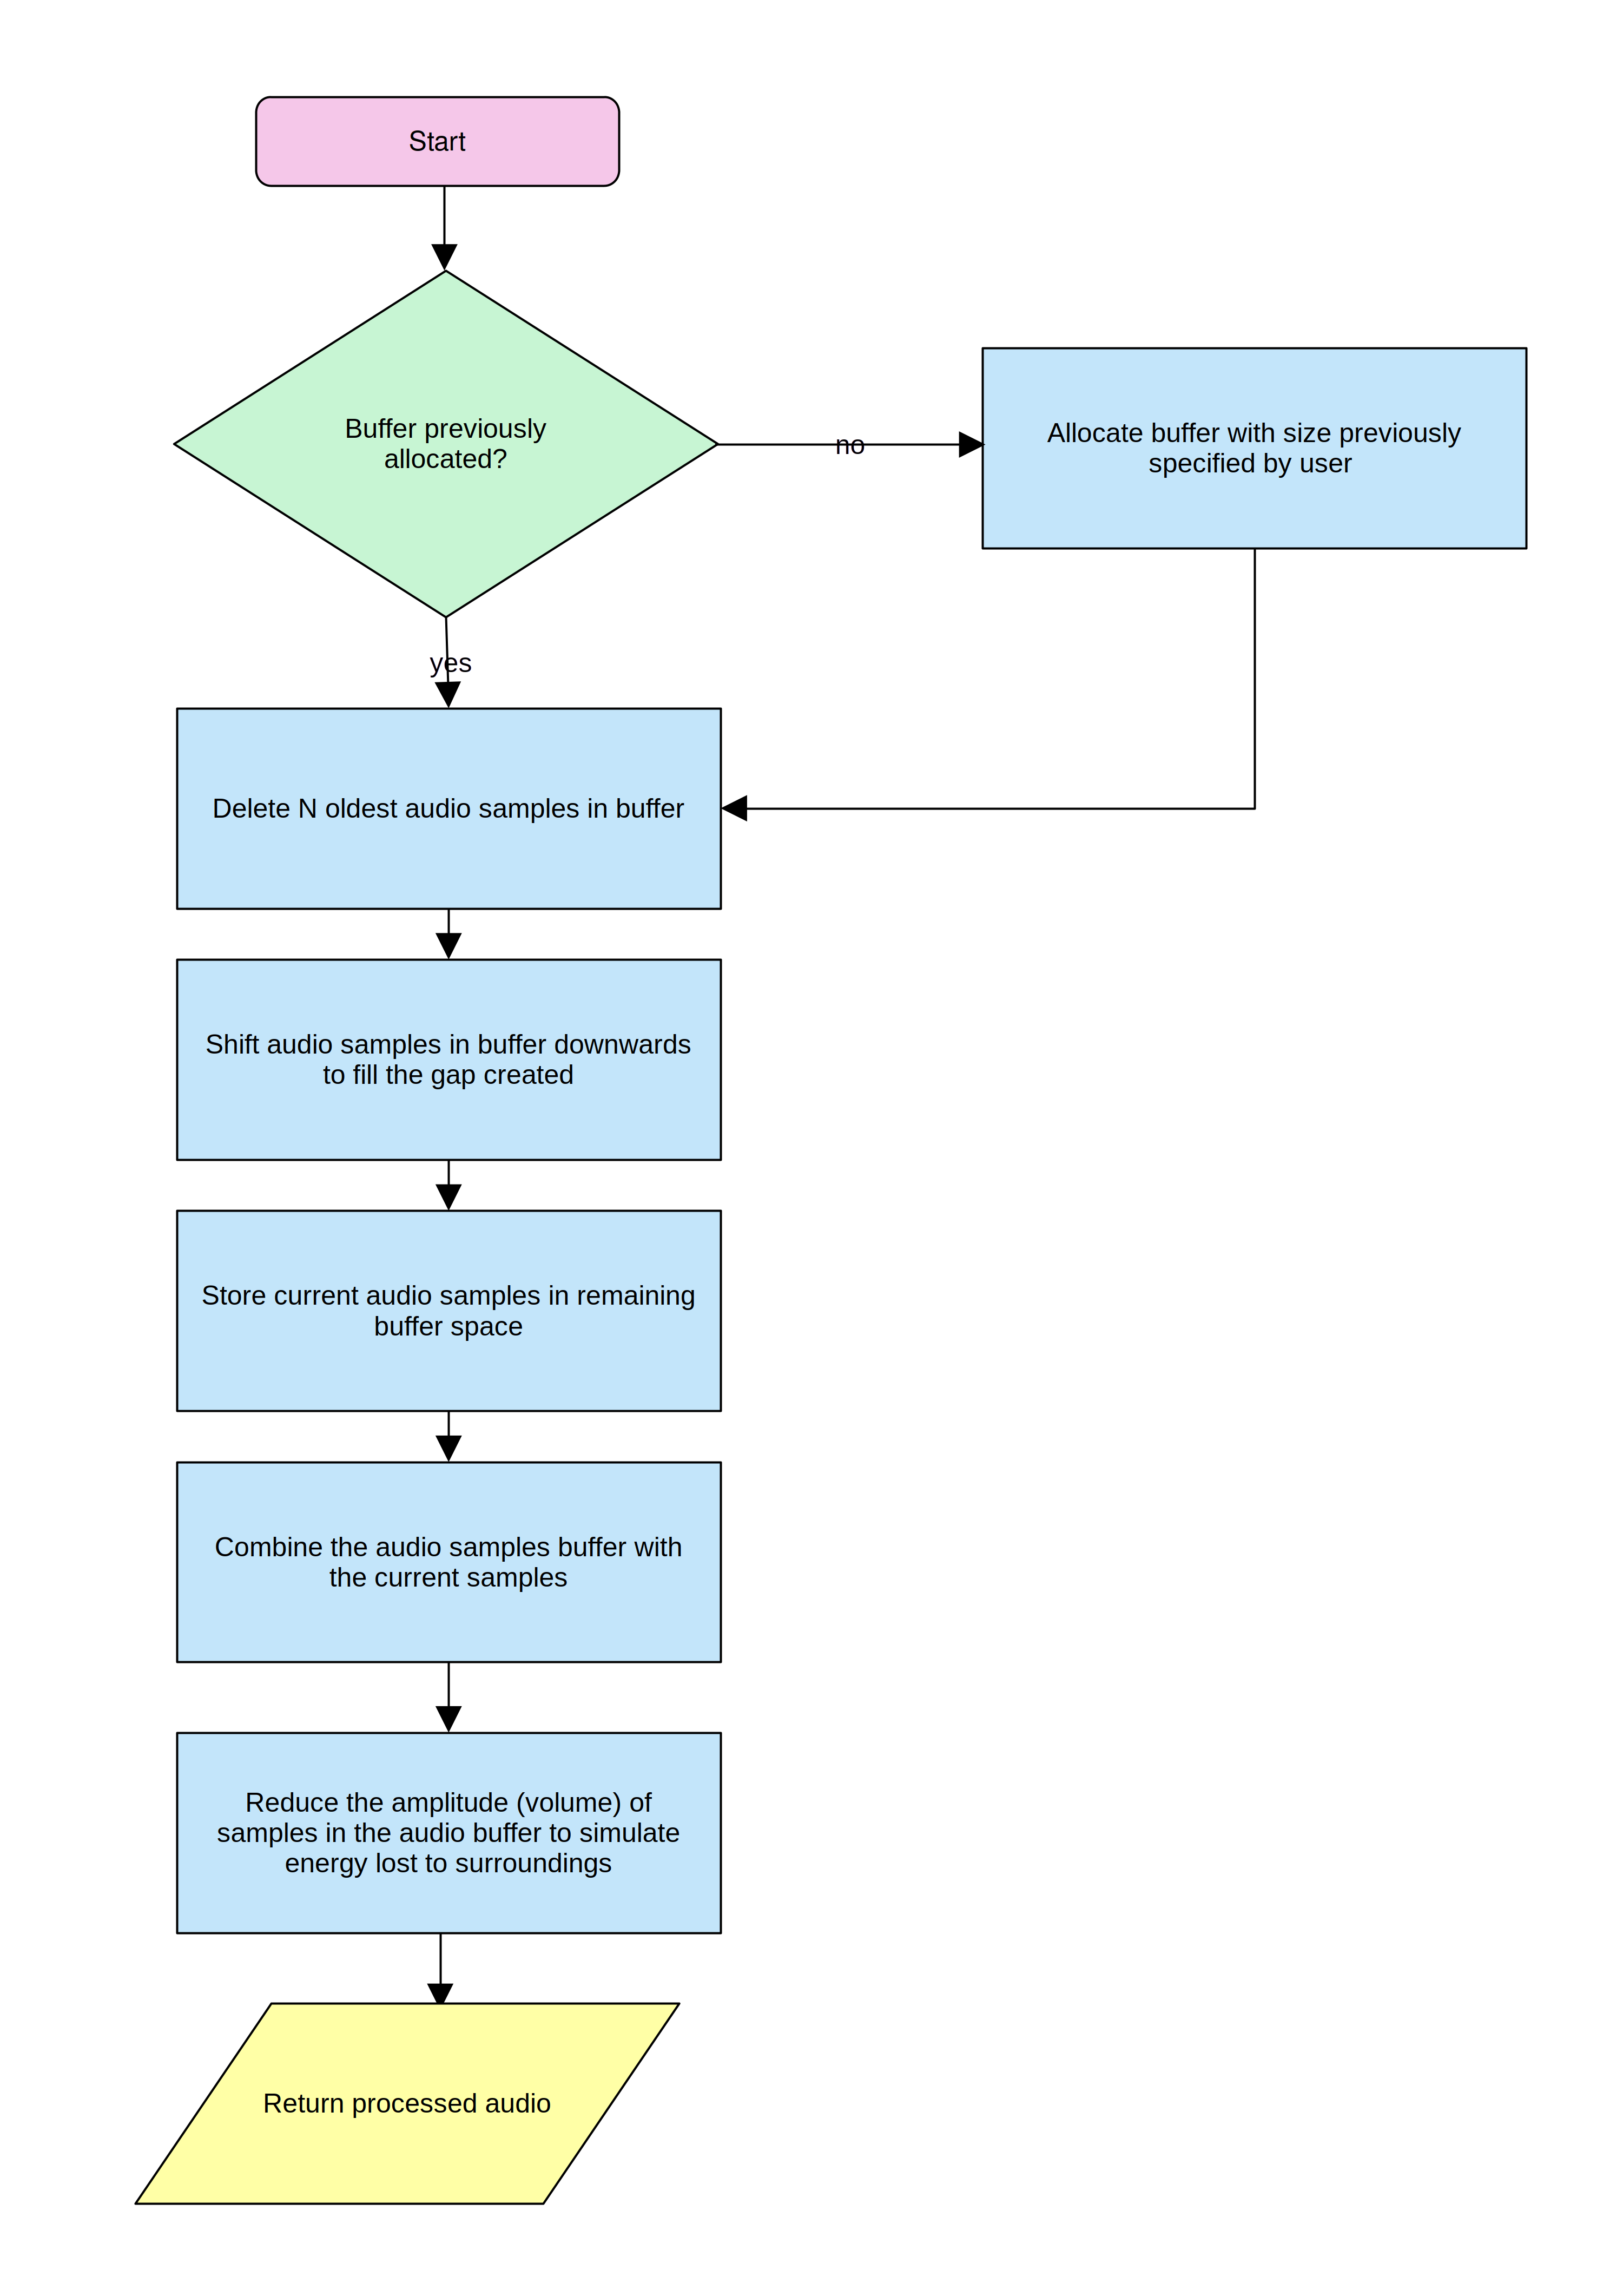
\includegraphics[width=14cm]{echo flowchart}
	\caption{Flowchart for echo audio effect}
\end{figure}

\begin{figure}[H]
	\subsubsection{Volume}
	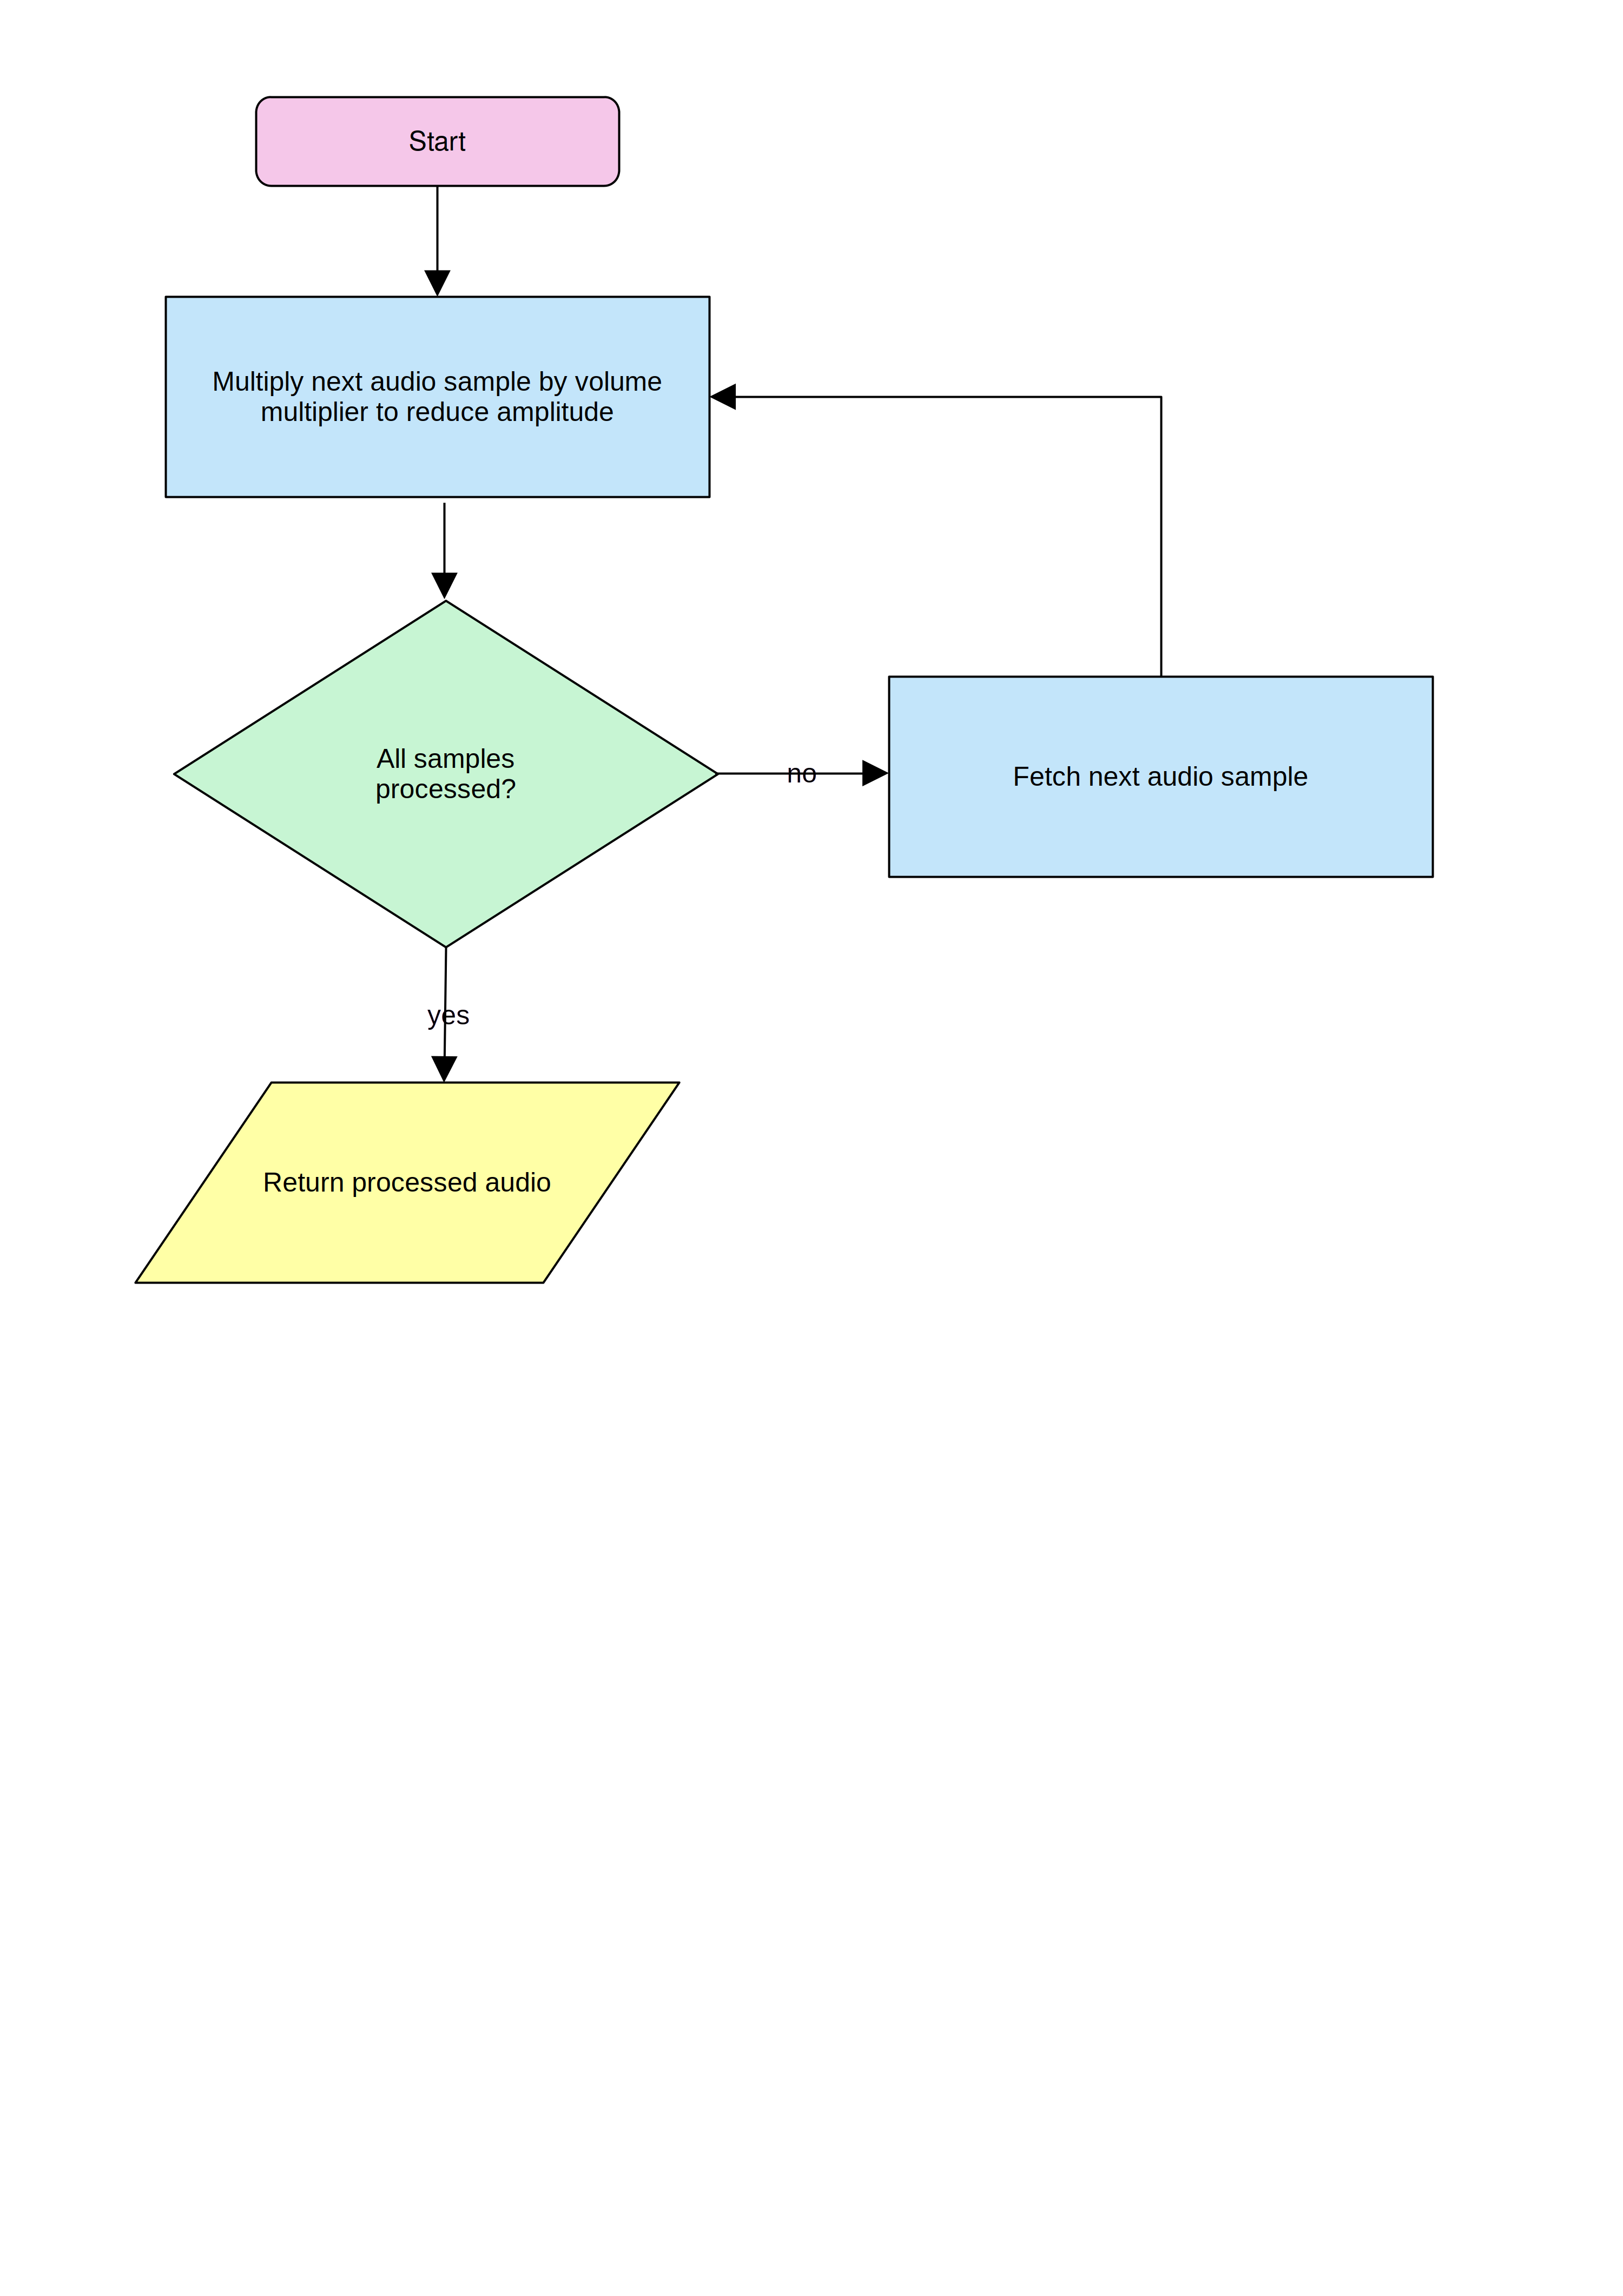
\includegraphics[width=14cm]{volume flowchart}
	\caption{Flowchart for volume audio effect}
\end{figure}

\begin{figure}[H]
	\subsubsection{Noise}
	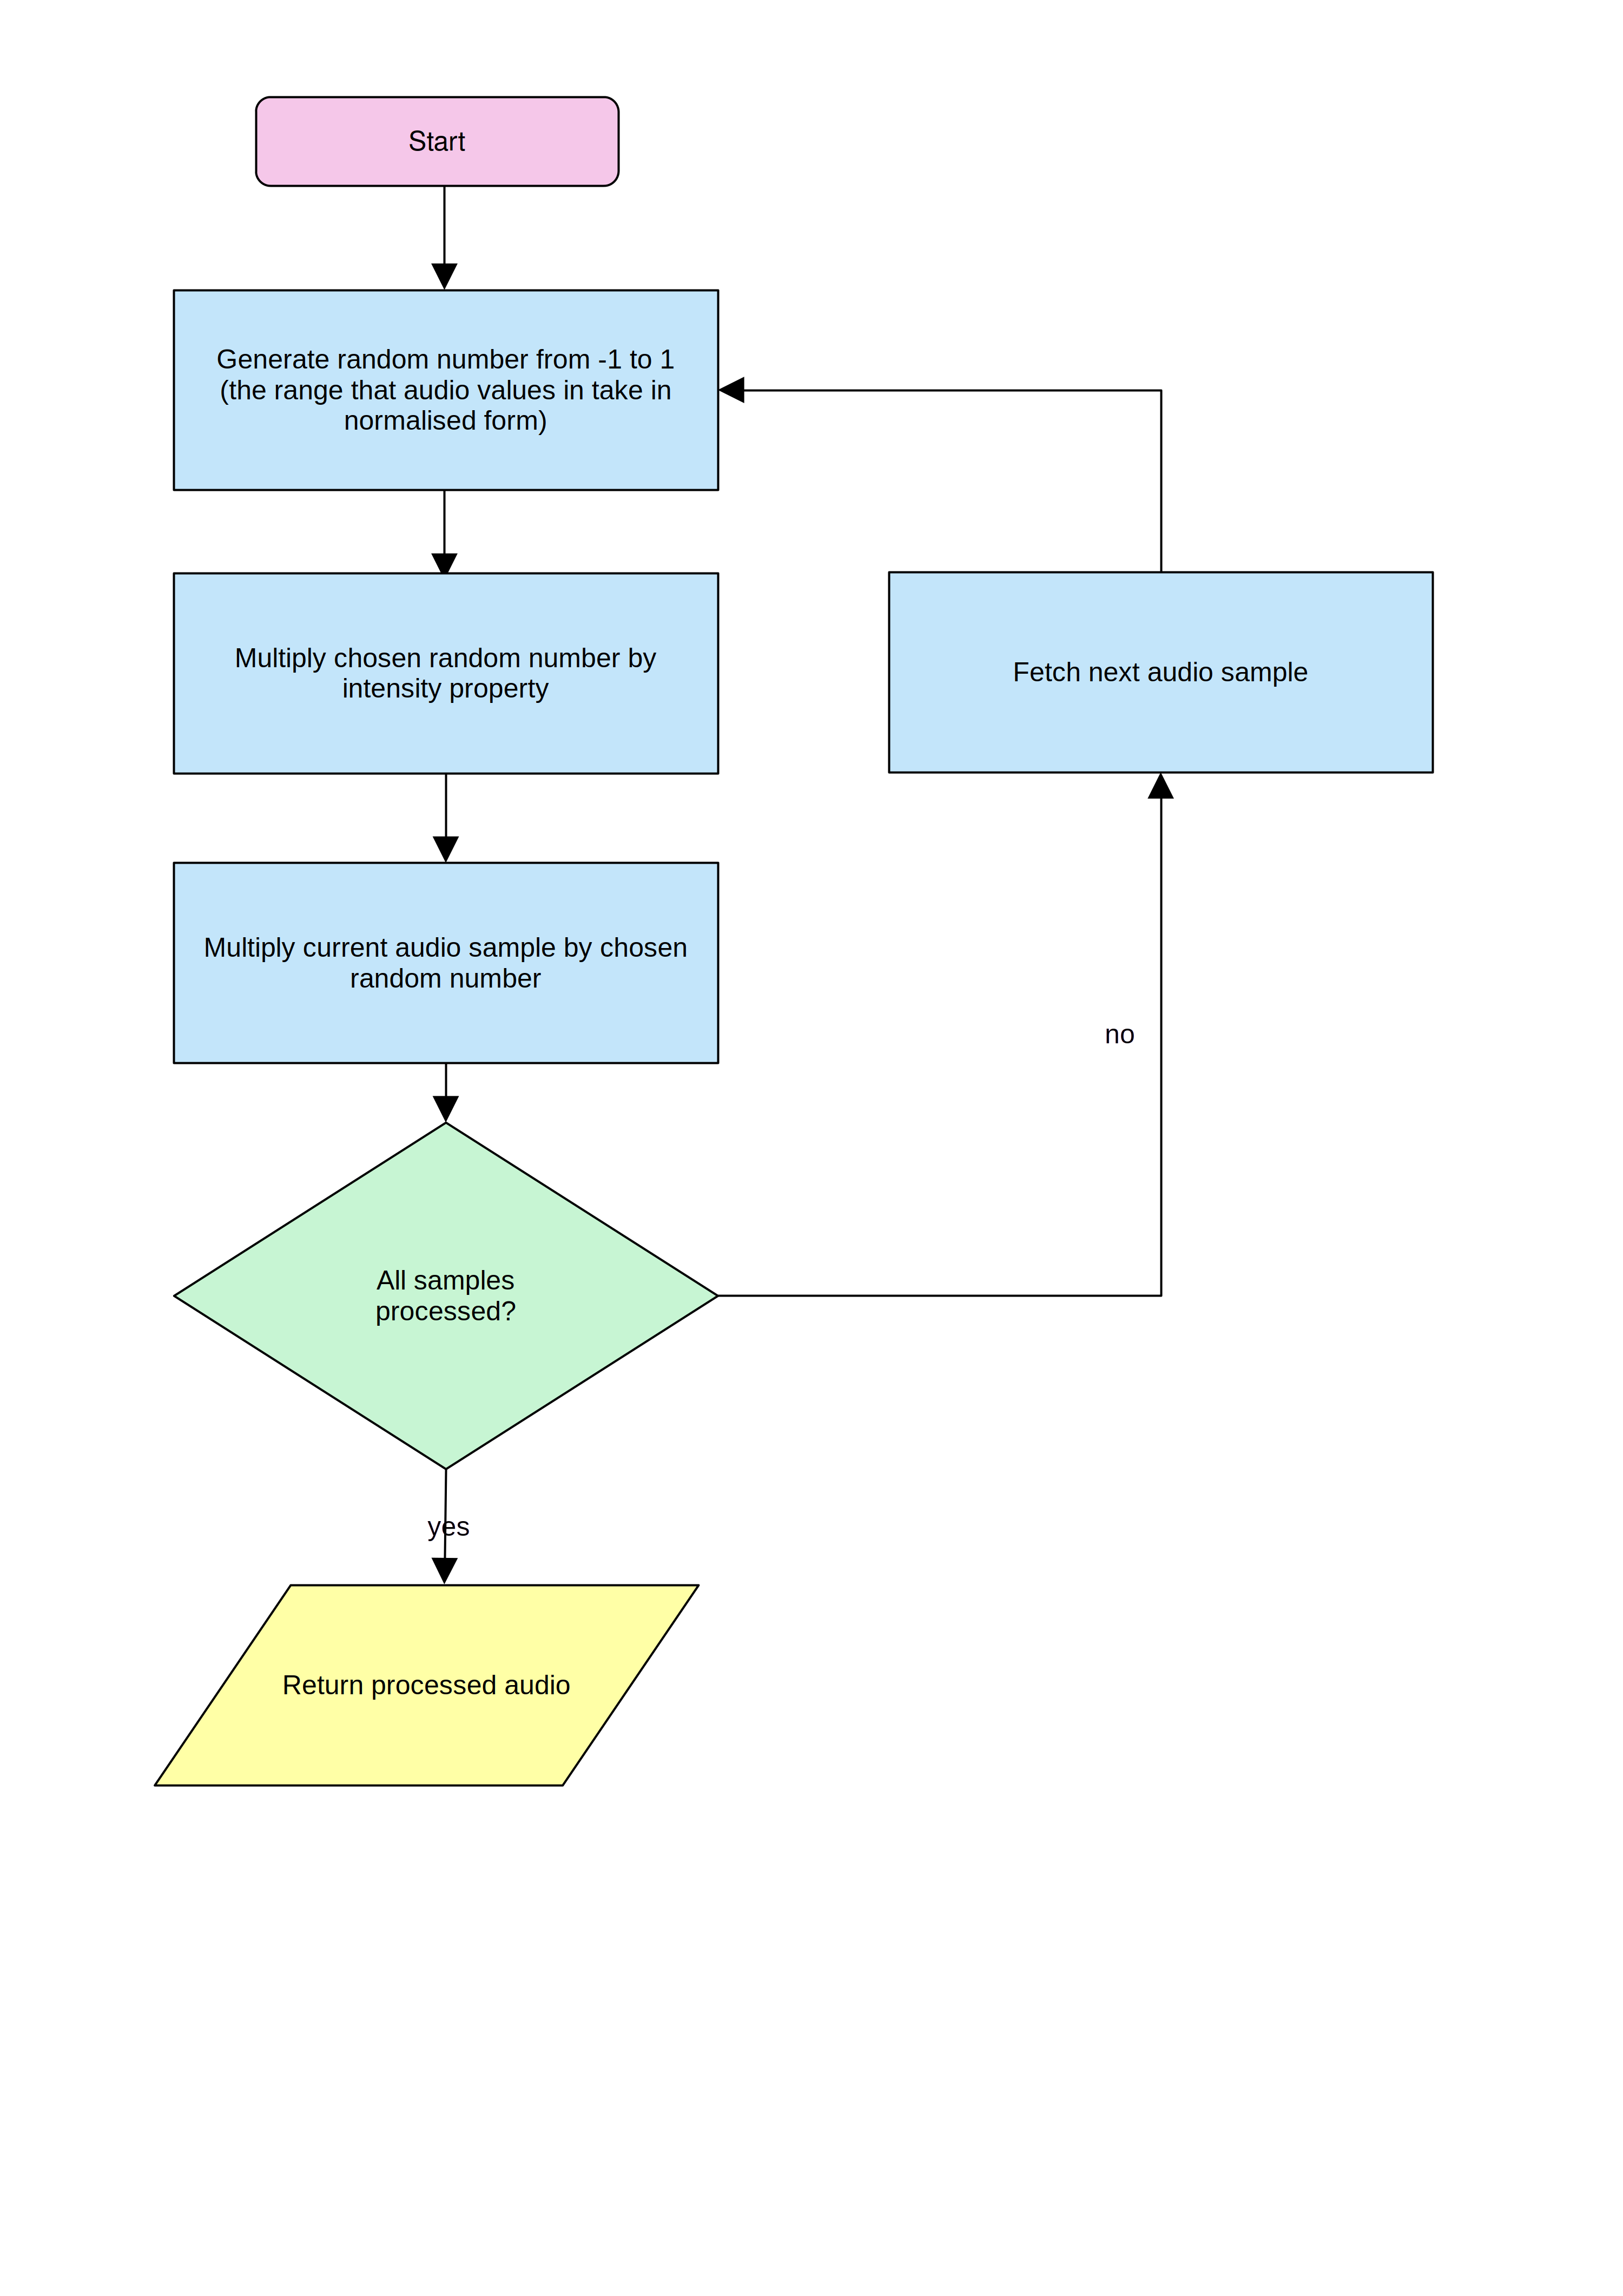
\includegraphics[width=14cm]{noise flowchart}
	\caption{Flowchart for noise audio effect}
\end{figure}

\pagebreak
\subsection{Final overview of project hierarchy}
\begin{figure}[H]
	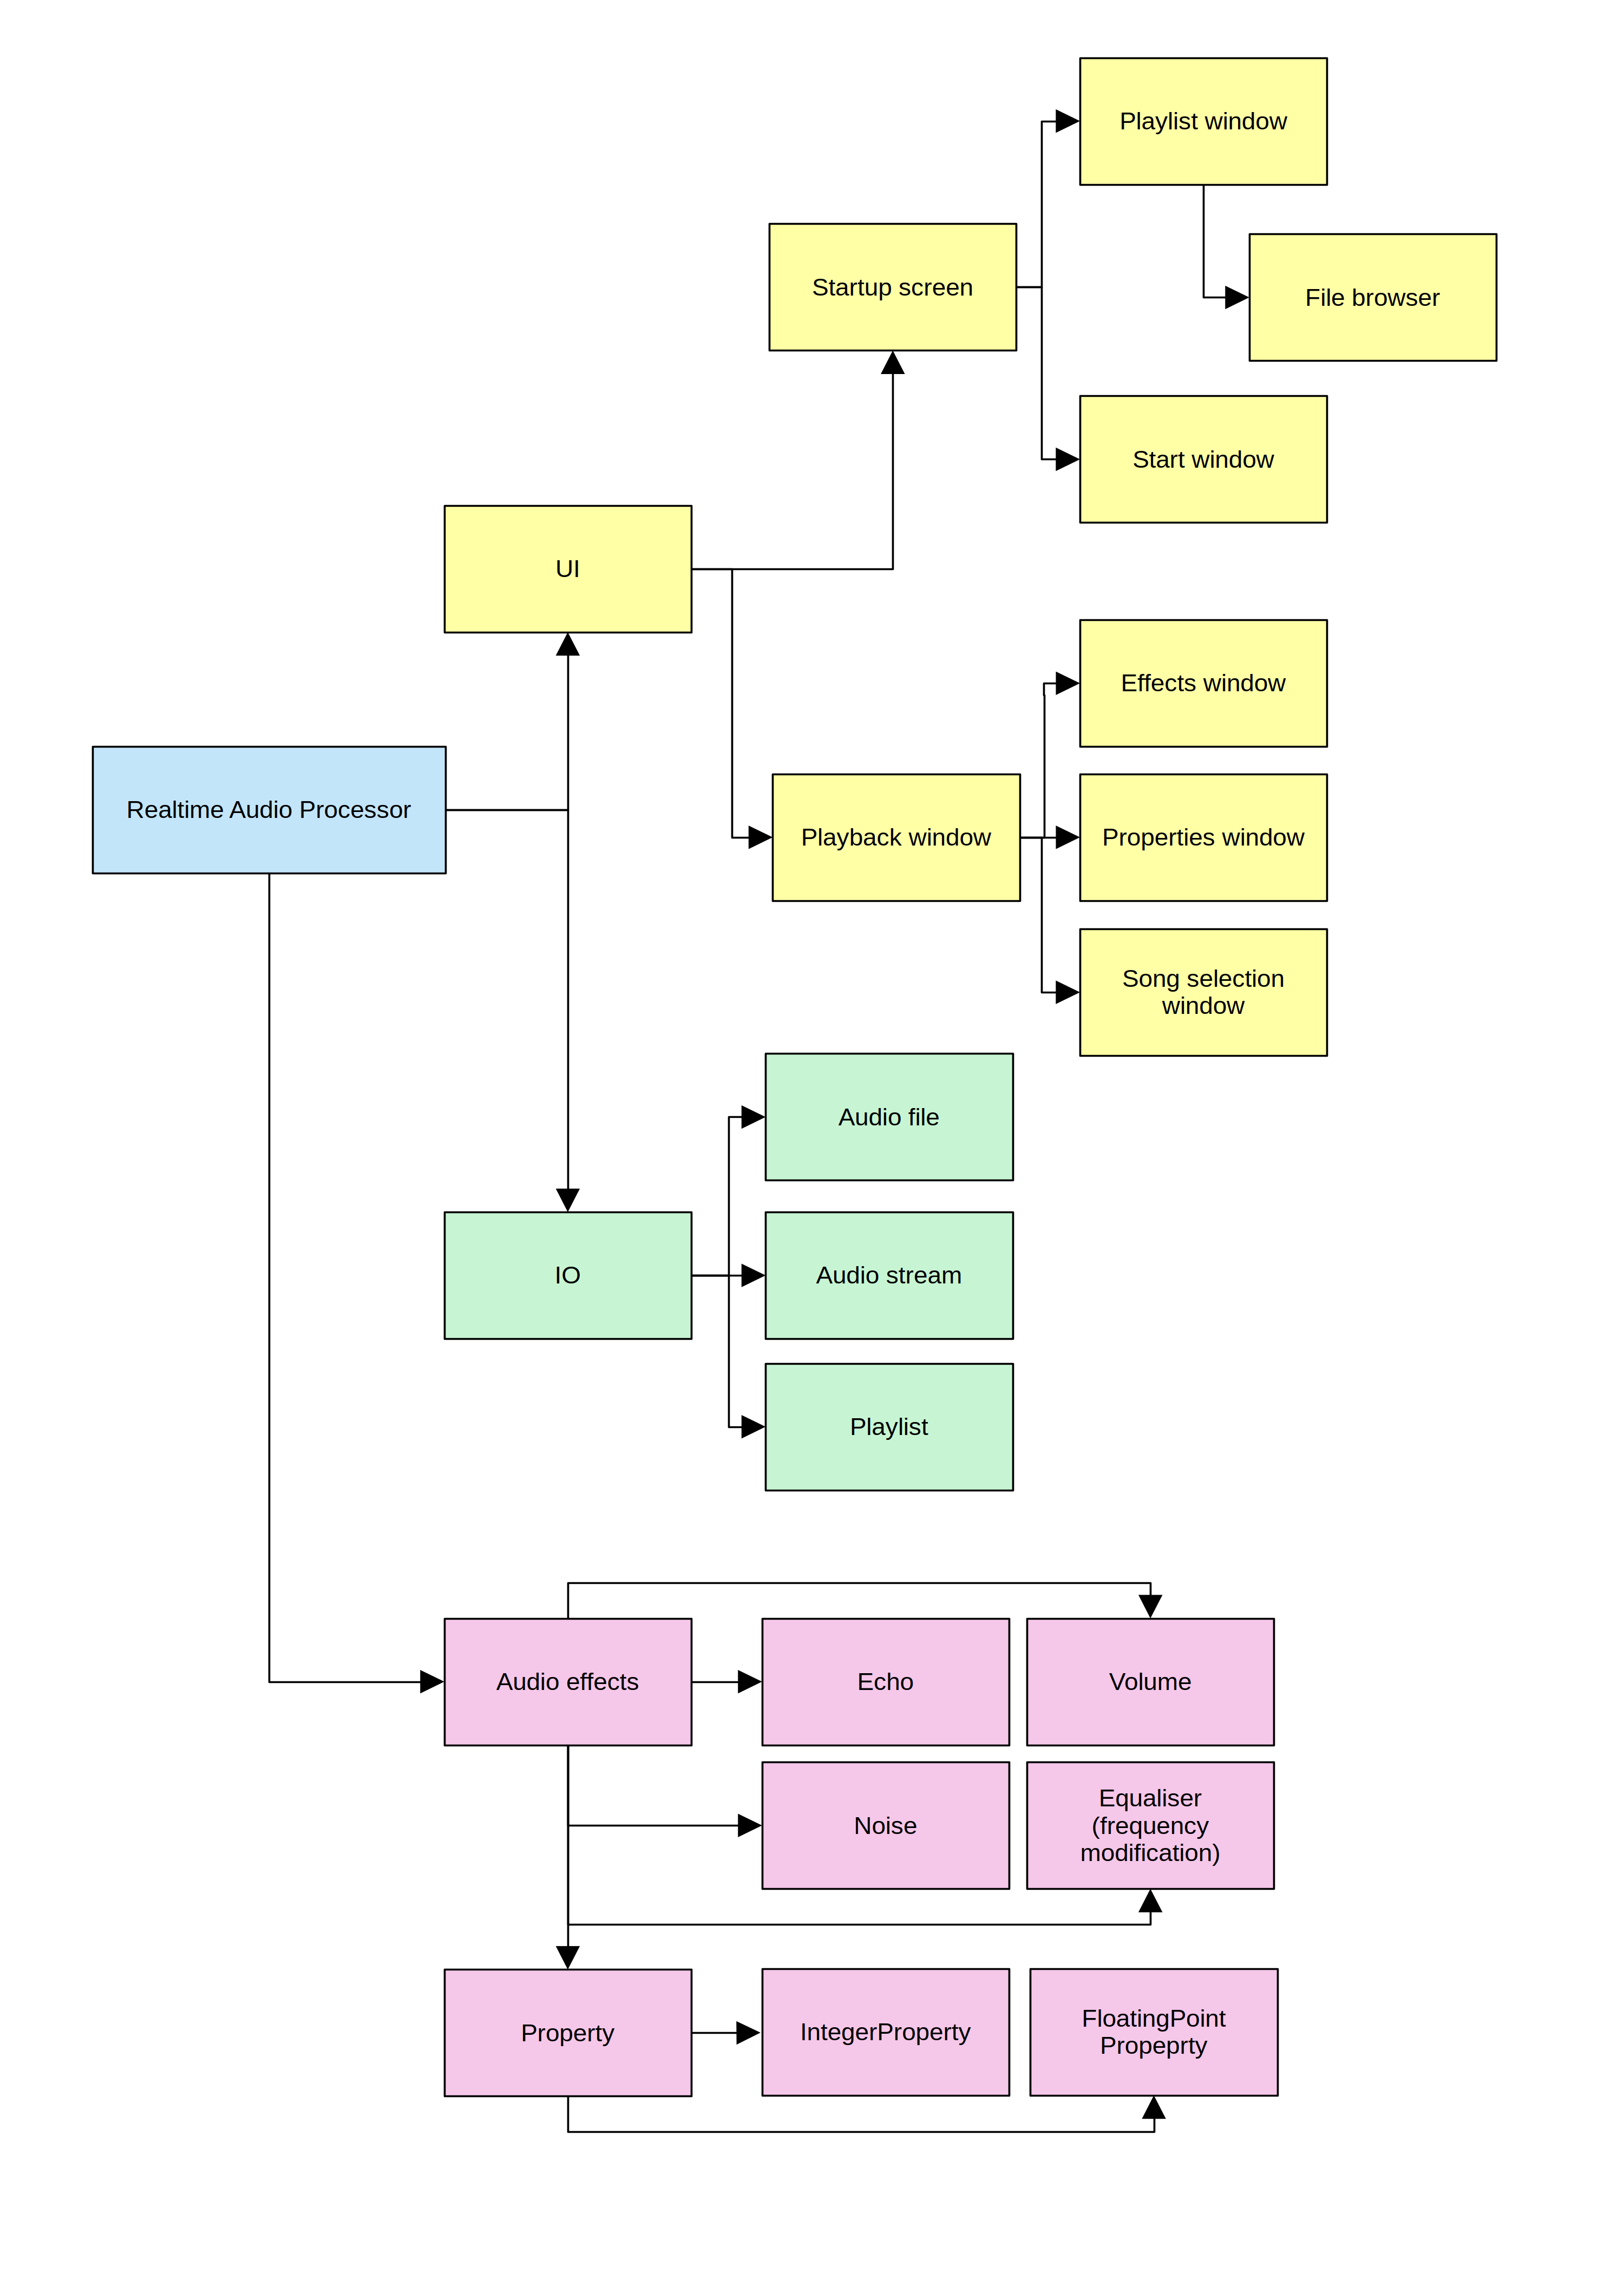
\includegraphics[width=14cm]{hierarchy chart}
	\caption{Hierarchy chart }
\end{figure}

\pagebreak
\subsection{TODO}
\begin{itemize}
	\item GUI design - i.e. wireframe
	\item Flow charts
	\item Test design
	\item Hierarchy chart (major components only)
	\item talk about IO classes
	\item talk about merge sort
	\item talk about atomic linked list
	\item talk about tree
\end{itemize}